\clearpage
\section{Vor dem Verwaltungsgebäude}
\label{sec:verwaltung-aussen}
\noindent\textbf{Abschnitt:} 1.2\quad
\textbf{Ort:} Veranda des Verwaltungsgebäudes\quad
\textbf{Zeit:} 5. April 1920, gegen 10 Uhr

\begin{center}
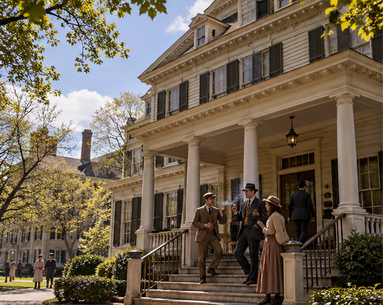
\includegraphics[width=.94\textwidth]{bilder/verwaltungsgebaeude-aussen.png}
\par\vspace{3pt}{\footnotesize\itshape Das Verwaltungsgebäude der Miskatonic University mit seiner gro\ss{}zügigen Veranda.}
\end{center}

\begin{vorlesetext}
Nach einem kurzen Spaziergang über die gepflegten Wege des Universitätsgeländes gelangst Du an einen kleinen, von alten Laubbäumen gesäumten Platz. Vor Dir erhebt sich ein stattliches, dreistöckiges Gebäude, das sich in seiner Architektur deutlich von den gewaltigen steinernen Fakultätsgebäuden unterscheidet.

Das Haus ist ganz im Stil der traditionellen amerikanischen Architektur gehalten. Seine breite Fassade besteht aus sorgfältig verarbeiteten, horizontal angebrachten Holzbrettern, deren ursprünglich cremewei\ss{}er Anstrich im hellen Sonnenlicht beinahe makellos erscheint. Hohe, regelmä\ss{}ig angeordnete Sprossenfenster mit dunkelgrünen Fensterläden verleihen dem Gebäude eine gewisse Strenge, die jedoch durch die gro\ss{}zügigen Proportionen und die zahlreichen architektonischen Verzierungen aufgelockert wird. Ein steiles, mit dunklen Schindeln gedecktes Dach schlie\ss{}t das oberste Geschoss ab. Mehrere gemauerte Schornsteine ragen darüber hinaus.

Eine breite, überdachte Veranda erstreckt sich über nahezu die gesamte Vorderseite des Hauses. Schlanke, wei\ss{} gestrichene Holzsäulen tragen das leicht geneigte Vordach. Zwischen ihnen verläuft ein aufwendig gearbeitetes Geländer, an dessen Fu\ss{} einige gro\ss{}e Terrakottatöpfe mit blühenden Pflanzen aufgestellt sind. Eine breite Holztreppe mit fünf flachen Stufen führt von dem gepflasterten Vorplatz hinauf zur Veranda.

Dort stehen drei junge Leute, zwei Herren und eine Dame, die sich offenbar angeregt unterhalten. Einer der Herren lehnt mit lässig verschränkten Beinen an einer der wei\ss{}en Säulen und hält eine brennende Zigarette zwischen den Fingern. Sein Begleiter, in einem hellbraunen Anzug und mit etwas zerzaustem Haar, gestikuliert lebhaft, während die junge Dame mit einem amüsierten Lächeln zuhört. Hin und wieder steigt eine dünne, bläuliche Rauchfahne empor, die sich langsam unter dem Verandadach verliert.

Das gedämpfte Knarren der hölzernen Dielen mischt sich mit ihren Stimmen und dem fernen Treiben des Campus. Als Du näher kommst, wendet einer der jungen Männer kurz den Kopf in Deine Richtung, schenkt Dir ein höfliches Nicken und setzt sein Gespräch fort.

Hinter der kleinen Gruppe befindet sich eine breite, dunkel lackierte Eingangstür mit zwei verglasten Flügeln. Das blank polierte Messing der Türgriffe glänzt im Sonnenlicht.
\end{vorlesetext}

\begin{meisterinfo}
\textbf{Situation.} Karim kann die Gruppe ansprechen, das Gebäude näher betrachten oder direkt eintreten. Eine Fertigkeitsprobe ist nicht erforderlich. Die drei Studierenden machen eine kurze Pause zwischen Veranstaltungen. Sie sind höflich, aber mit ihrem Gespräch beschäftigt.

\medskip
\textbf{Frage: Ist dies das Verwaltungsgebäude?}

\emph{\glqq{}Ja, ganz richtig. Hier sind Sie bei der Verwaltung. Wenn Sie jemanden suchen, wenden Sie sich am besten gleich an den Empfang. Direkt hinter der Eingangstür, Sie können ihn gar nicht verfehlen.\grqq{}}

\medskip
\textbf{Frage: Wo ist der Universitätspräsident?}

\emph{\glqq{}Zum Präsidenten? Dann haben Sie jedenfalls das richtige Gebäude gefunden. Sein Büro liegt irgendwo oben. Der Herr am Empfang wird Ihnen sicher weiterhelfen können.\grqq{}}

\medskip
\textbf{Frage: Muss ich mich anmelden?}

\emph{\glqq{}Das würde ich Ihnen empfehlen. Die Herren hier legen ziemlich gro\ss{}en Wert auf solche Dinge.\grqq{}}

\medskip
\textbf{Frage: Kennen Sie Professor Garmond?}

\emph{\glqq{}Professor Garmond? Ein vielbeschäftigter Mann. Man bekommt ihn nicht gerade häufig zu Gesicht. Aber wenn Sie einen Termin haben, werden Sie wohl schon erwartet.\grqq{}}

\medskip
\textbf{Grenze ihres Wissens.} Die Studierenden wissen nichts über die verschwundene Expedition. Bei weiteren Fragen verweisen sie auf den Empfang.

\textbf{Übergang.} Sobald Karim die Eingangstür öffnet, beginnt Abschnitt 1.3.
\end{meisterinfo}

\clearpage
\section{Die Eingangshalle der Universitätsverwaltung}
\label{sec:verwaltung-innen}
\noindent\textbf{Abschnitt:} 1.3\quad
\textbf{Ort:} Eingangshalle und Empfang\quad
\textbf{Zeit:} 5. April 1920, gegen 10 Uhr

\begin{center}
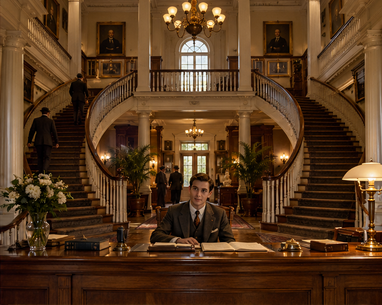
\includegraphics[width=.94\textwidth]{bilder/verwaltung-eingangshalle.png}
\par\vspace{3pt}{\footnotesize\itshape Die Eingangshalle mit dem Empfangstresen zwischen den beiden Treppenaufgängen.}
\end{center}

\begin{vorlesetext}
Du drückst einen der schweren Messinggriffe herunter und öffnest die Eingangstür. Mit einem leisen Knarren schwingt der Türflügel nach innen, und Du trittst über die Schwelle.

Du findest Dich in einer überraschend gro\ss{}en, lichtdurchfluteten Halle wieder. Die hohen Decken und gro\ss{}zügigen Abmessungen des Raumes lassen das Gebäude von innen noch eindrucksvoller erscheinen, als es von au\ss{}en ohnehin schon gewirkt hat.

Der Boden besteht aus gro\ss{}en, hellgrauen Natursteinplatten, die sorgfältig geschliffen wurden und im einfallenden Tageslicht einen matten Glanz zeigen. Ein breiter, dunkelroter Teppichläufer führt vom Eingangsbereich geradewegs zu einem mächtigen Empfangstresen aus dunkel gebeiztem Eichenholz.

Links und rechts erheben sich zwei breite, elegant geschwungene Holztreppen. Ihre polierten Geländer folgen in weiten Bögen den Treppenläufen hinauf zu einer offenen Galerie im ersten Obergeschoss, von der aus weitere Treppen in die darüberliegenden Stockwerke führen. Die Treppenstufen sind mit schmalen Teppichläufern belegt, die von blanken Messingstangen gehalten werden.

Die Wände der Halle sind im unteren Bereich mit dunklem Holz vertäfelt. Darüber hängen mehrere gro\ss{}e Ölgemälde in schweren, vergoldeten Rahmen, die würdevoll dreinblickende Herren in akademischer Kleidung zeigen. Vermutlich frühere Präsidenten oder andere bedeutende Persönlichkeiten der Universität.

Ein mächtiger Kronleuchter aus Messing und geschliffenem Glas hängt von der hohen Decke herab. Obwohl seine elektrischen Lampen nicht eingeschaltet sind, fällt durch die hohen Fenster genügend Sonnenlicht in den Raum, um selbst die entferntesten Winkel zu erhellen.

Hinter dem Empfangstresen sitzt ein junger Mann von vielleicht fünfundzwanzig Jahren. Er trägt einen tadellos sitzenden dunkelgrauen Anzug, eine schmale Krawatte und eine sorgfältig frisierte, seitlich gescheitelte Frisur. Neben ihm stehen ein Telefonapparat mit getrenntem Hörer, mehrere Ablagekörbe und ein kleiner Stapel Schriftstücke.

Als Du eintrittst, ist er gerade damit beschäftigt, einige Eintragungen in einem gro\ss{}en, ledergebundenen Buch vorzunehmen. Er führt seinen Füllfederhalter mit schnellen, geübten Bewegungen über das Papier.

Beim Geräusch der zufallenden Eingangstür hält er inne. Er legt den Füllfederhalter sorgfältig neben das aufgeschlagene Buch, hebt den Kopf und blickt Dir mit einem freundlichen, aber professionellen Lächeln entgegen.
\end{vorlesetext}

\begin{meisterinfo}
\textbf{Empfangsmitarbeiter.} Der junge Angestellte ist höflich, gewissenhaft und darauf bedacht, Besucher zu ihren Ansprechpartnern zu leiten. Er verhält sich freundlich, aber bestimmt.

\medskip
\textbf{Karim tritt zum Tresen:}

\emph{\glqq{}Guten Morgen, mein Herr. Herzlich willkommen in der Miskatonic University. Was kann ich für Sie tun?\grqq{}}

\medskip
\textbf{Karim erwähnt seinen Termin bei Präsident Garmond:}

\emph{\glqq{}Selbstverständlich, mein Herr. Dürfte ich zunächst um Ihren Namen bitten?\grqq{}}

Nachdem Karim seinen Namen genannt hat, prüft der Mann das Besucherbuch.

\emph{\glqq{}Ah, Herr el-Mady. Ja, hier habe ich Sie. Sie werden um elf Uhr bei Professor Garmond erwartet.\grqq{}}

Er schaut auf eine Standuhr hinter dem Tresen.

\emph{\glqq{}Sie sind erfreulich früh eingetroffen. Das Büro des Präsidenten befindet sich im zweiten Obergeschoss. Nehmen Sie bitte die linke Treppe und folgen Sie ihr bis ganz nach oben. Dort halten Sie sich rechts. Am Ende des Korridors finden Sie das Vorzimmer des Präsidenten. Seine Sekretärin wird Sie dort in Empfang nehmen.\grqq{}}

\medskip
\textbf{Frage: Darf ich bereits hinaufgehen?}

\emph{\glqq{}Aber selbstverständlich. Ich bin sicher, dass man Ihnen im Vorzimmer eine Sitzgelegenheit anbieten kann.\grqq{}}

\medskip
\textbf{Karim versucht, wortlos vorbeizugehen:}

Der junge Mann erhebt sich leicht von seinem Stuhl.

\emph{\glqq{}Verzeihen Sie bitte, mein Herr. Darf ich erfahren, wen Sie zu besuchen wünschen? Ich bin Ihnen gerne behilflich.\grqq{}}

Er hindert Karim nicht körperlich am Weitergehen.

\medskip
\textbf{Frage: Wie ist Professor Garmond?}

\emph{\glqq{}Professor Garmond ist ein au\ss{}erordentlich beschäftigter Mann, wie Sie sich sicher vorstellen können. Aber er legt gro\ss{}en Wert darauf, seine vereinbarten Termine persönlich wahrzunehmen.\grqq{}}

\medskip
\textbf{Spielhinweis.} Hier sind keine Fertigkeitsproben erforderlich. Der Mitarbeiter kennt den genauen Zweck des Termins und die Hintergründe der Expedition nicht, wei\ss{} aber, dass mehrere Gäste für elf Uhr erwartet werden.

\textbf{Übergang.} Sobald Karim zum zweiten Obergeschoss aufsteigt, beginnt der Abschnitt im Vorzimmer des Präsidenten. Dort treffen die vier Ermittler zusammen.
\end{meisterinfo}
